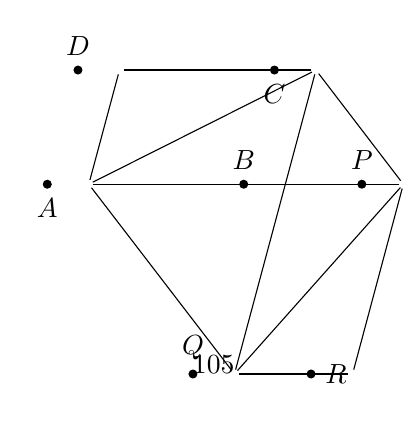
\begin{tikzpicture}
[scale =0.5,>=stealth,point/.style = {draw, circle, fill = black, inner sep = 1pt},]
\node (D) at (-2.92,7.72)[point,label=above :$D$] {};
\node (C) at (2.07,7.72)[point,label=below :$C$] {};
\node (A) at (-3.70,4.82)[point,label=below :$A$] {};
\node (B) at (1.29,4.82)[point,label=above :$B$] {};
\node (P) at (4.29,4.82)[point,label=above :$P$] {};
\node (Q) at (0,0)[point,label=above :$Q$] {};
\node (R) at (3,0)[point,label=right :$R$] {};
\tkzMarkAngle[fill=red!105,size=.4,mark=](C,R,Q)
\tkzLabelAngle[pos=0.75](C,R,Q){$105\degree$}

\draw (A)--(P);
\draw (C)--(P);
\draw (Q)--(C);
\draw (C)--(D);
\draw (D)--(A);
\draw (P)--(R);
\draw (C)--(A);
\draw (P)--(Q);

\draw (R)--(Q);
\draw (A)--(Q);
\end{tikzpicture}
